% !TeX program = latexmk
%%%
%%% LaTeX 2e (mostly) version of TTU thesis and dissertation format
%%% by Mike Renfro (renfro at tntech.edu) et al
\documentclass[copyrighted]{ttuthesis}

\title{Guide to the Preparation of\\Theses and Dissertations}
\author{Jan R. Doe}
\doctype{Thesis}
\degree{Master of Science}
\department{Electrical Engineering}
\graduationmonth{May}
\graduationyear{1993}
\hypersetup{
  pdfsubject={Format and style rules for theses and dissertations at Tennessee Technological University},
  pdfkeywords={thesis, dissertation, style guide}
}
\abstract{%
  This manual was designed to guide you in the preparation of your
  thesis or dissertation at Tennessee Technological University. It is
  adapted from the Tennessee Conference of Graduate Schools
  \textit{Guide to the Preparation of Theses and Dissertations}
  \cite{lacava1992} and the \textit{Tennessee Technological University
  Thesis Manual} \cite{ttu1989}. Following the practice of many
  guides and manuals, it is written in the second person, addressed
  directly to the reader. You should understand, however, that the
  second person is generally not appropriate usage in a thesis or
  dissertation.

  Appreciation is extended to the authors of the manual: Dr. Suellen
  Alfred, Dr. Frank Bulow, Dr. Helen Deese, Mrs. Sheila Kendrick, Dr.
  Ken Purdy, and Dean Rebecca Quattlebaum.
}
\dedication{%
  \begin{center}
    This thesis is dedicated to my parents \\
    who have given me invaluable educational opportunities.     
  \end{center}
}
\acknowledgments{%
  Appreciation is extended to the authors of the manual: Dr. Suellen
  Alfred, Dr. Frank Bulow, Dr. Helen Deese, Mrs. Sheila Kendrick, Dr.
  Ken Purdy, and Dean Rebecca Quattlebaum.
}
\committeechair{Chair's Name}
\committeecochair{Cochair's Name}
\committeemembers{Member 1's Name, Member 2's Name}

\begin{document}
\begin{Spacing}{1}
\tableofcontents*
\listoftables
\listoffigures
\renewcommand{\nomname}{LIST OF SYMBOLS} \printnomenclature
\end{Spacing}
% Main matter
\mainmatter
\chapter{The Essentials}
\label{chap:TheEssentials}

\section{Purpose of the Guide}
\label{sec:PurposeOfTheGuide}

This guide is designed to be a basic source of information for
the\-sis/dis\-ser\-ta\-tion preparation. It establishes the technical
parameters within which you should work, such as quality of paper,
number of copies to be submitted, margins, and the sequence of pages
within the manuscript. Since most of you will publish during and after
your graduate education, this guide encourages the use of leading
professional publications to help establish specific formatting
convention. You are encouraged to use publications within your
field---journals and textbooks---to assist you in establishing
bibliographic form, use of number, and other conventions that are
discipline oriented.  However, the application of this theory is not
simple. You must understand the various elements of a manuscript and
general publication formatting requirements in academic publishing.
Although knowledge and use of publication formatting is essential, the
regulations established by this guide always take precedence.

You should use style handbooks such as the most recent editions of the
\textit{MLA Handbook for Writers of Research Papers} (English)
\cite{gibaldi1988}, \textit{Publication Manual of the American
  Psychological Association} (Education) \cite{apa1983}, \textit{CBE
  Style Manual (Biology)} \cite{cbe1983}, \textit{Form and Style}
(Arts \& Sciences, Engineering, Education) \cite{campbell1990},
\textit{The Chicago Manual of Style} \cite{chicago1982}, and
\textit{Harbrace College Handbook} \cite{hodges1990} as resources for
basic style and grammar. In contrast, you should never use previously
accepted theses and dissertations as the final guide to style.
Examples taken from other theses may be out of context or may be
incorrect. The existence of a particular style or usage in a
previously accepted thesis does not establish a precedent for its
continuation.
% The following two nomenclature entries are intended for the thesis manual.
% Best practice is to add \nomenclature commands with first use of a term.
\nomenclature{MLA}{Modern Language Association}
\nomenclature{CBE}{Council of Biological Editors}

By accepting your thesis or dissertation and awarding the degree,
Tennessee Technological University places its academic reputation on
the line. The content of your manuscript is carefully evaluated by
experts in your field. The format requirements presented in this guide
are imposed to ensure an appropriate academic appearance of your
manuscript.


\section{Ethical Standards}
\label{sec:EthicalStandards}

Since conferral of a graduate degree implies professional integrity
and knowledge of scholarly methods, there are three areas in which you
as a graduate student should be particularly cautious:

\begin{itemize}
\item proper acknowledgment of cited works
\item the proper use of copyrighted material
\item the proper reporting of work where research compliance is required
\end{itemize}

\subsection{Plagiarism}
\label{sec:Plagiarism}

\textit{Merriam-Webster's Collegiate Dictionary} \cite{webster1993}
defines plagiarism as ``steal\-[ing] and pass\-[ing] off ideas or
words of another as one's own'' and ``the use of a created production
without crediting the source.'' ``You must acknowledge all material
quoted, paraphrased, or summarized from any published or unpublished
work.  Failing to cite a source, deliberately or accidentally, is
plagiarism'' \cite[424]{webster1993}. If you use the exact words of
your source, they must be enclosed in quotation marks and the source
cited; if you do not use the exact words but paraphrase or summarize
the source, it still must be cited.  When involved in collaborative
research, you should exercise extreme caution to avoid questions of
plagiarism. If in doubt, check with your major professor and the
Graduate School about the project. Plagiarism will be investigated
when suspected and prosecuted if established.


\subsection{Copyright}
\label{sec:Copyright}

If you use copyrighted material in a limited way, it is usually
unnecessary to seek permission to quote. If, however, you use material
from a copyrighted work to the extent that the rights of the copyright
owner might be violated, you must obtain permission of the owner. In
determining the extent of a written work that may be quoted without
permission, you should consider the proportion of the material to be
quoted in relation to the substance of the entire work. According to
\textit{The Chicago Manual of Style} \cite{chicago1982}, ``A few lines
from a sonnet, for instance, form a greater proportion of the work
than do a few lines from a novel. Use of anything in its entirety is
hardly ever acceptable'' (p. 124). In no case should you copy a
standardized test of similar material and include it in a
the\-sis/dis\-ser\-ta\-tion without written permission. According to
Circular 21 (Reproduction of Copyrighted Works by Educators and
Librarians, p. 11) \cite{loc1988}, ``\textellipsis{}the following
shall be prohibited: \textellipsis{} There shall be no copying of or
from works intended to be `consumable' in the course of study or of
teaching.  These include workbooks, exercises, standardized tests and
test booklets and answer sheets and like consumable material.'' The
publisher usually has the authority to grant permission to quote
excerpts from the copyrighted work or can refer requests to the
copyright owner or designated representative.  The copyright owner may
charge for permission to quote. You should credit permissions with the
acknowledgments, and the source should appear in the
Bibliography\footnote{Some fields alternatively use Literature Cited,
  References, or Works Cited.}.


\subsection{Federal and State Regulations}
\label{sec:FederalAndStateRegulations}

Compliance with federal and state regulations governing the use of
human subjects, animal care, radiation, legend drugs, recombinant DNA,
or the handling of hazardous materials/wastes in research is monitored
by a number of regulatory agencies. Because of these regulations,
research compliance is another area of importance to you as a graduate
student and to the conduct of your research. Tennessee Technological
University requires you to verify that you have complied with the
appropriate approval procedure(s) prior to the initiation of the
thesis- or dissertation-related research, if approval is relevant to
the research. If your research involves any of the areas mentioned
above, you should determine what compliance is required by the school
(available in the Office of Research).


\section{Definitions}
\label{sec:Definitions}


\subsection{Typeface or Font}
\label{sec:DefTypefaceOrFont}

These terms apply to all the features available within a ``type''
family. For many printers, typeface includes bold, italic, and the
various sizes of any named type (Helvetica, Times Roman, New York,
Geneva, etc.).


\subsection{Text}
\label{sec:DefText}

In the discussion of formatting, text is used as a generic term to
designate the main body of the the\-sis/dis\-ser\-ta\-tion and to
distinguish this element from preliminary pages, references, tables,
figures, and appendices.


\subsection{Preliminary Pages}
\label{sec:DefPreliminaryPages}

Sometimes called ``front matter,'' preliminary pages serve as a guide
to the contents and nature of the manuscript \cite{chicago1982}. The
approval or acceptance sheets, as part of the preliminary pages,
confirm acceptance by the committee members acting for the department,
and the Dean of Graduate Studies, acting for the university or
college.


\subsection{Table}
\label{sec:DefTable}

A table consists of numbers, words, or both, and presents information
that is separated into columns. Tabular information allows you, the
author, to convey information to a reader in a structured format.


\subsection{Figure}
\label{sec:DefFigure}

Any diagram, drawing, graph, chart, map, photograph, or material that
does not fit into the restricted format for a table is a figure.
Figures generally show relationships or illustrate information rather
than present precise data.


\subsection{Appendix}
\label{sec:DefAppendix}

An appendix is generally a ``catch-all'' for supplementary material to
the the\-sis/dis\-ser\-ta\-tion. In some cases, tables and/or figures
are placed in an appendix to avoid interrupting the text. An example of an appendix can be seen in Appendix~\ref{chap:sample_tables}.

%%% Local Variables: 
%%% mode: latex
%%% TeX-master: "thesis"
%%% End: 

\chapter{Thesis/Dissertation Elements and Style}
\label{chap:Thesis/DissertationElementsAndStyle}

\section{Preliminary Pages}
\label{sec:PreliminaryPages}

Figure \ref{fig:ArrangementOfThesisParts} shows the sequence and
numbering scheme of the various the\-sis/dis\-ser\-ta\-tion parts.
Samples of all preliminary pages can be found at the start of this
document.
\begin{figure}[tbp]
  \centering
% Original version of table
%  \begin{tabular}{|p{3.0in}|p{2.0in}|} \hline
%    \textit{Thesis/Dissertation Parts} & \textit{Page Assignment} \\ \hline \hline
%    \textbf{Abstract} & No page number assigned \\ \hline
%    \textbf{Title Page} & Small Roman numeral (Assigned, not typed) \\ \hline
%    Copyright Page & \multirow{9}{*}{Small Roman numeral (Typed)} \\ \cline{1-1}
%    \textbf{Approval Sheet} & \\\cline{1-1}
%    \textbf{Statement of Permission to Use} (Master's theses only) & \\ \cline{1-1}
%    Dedication page & \\ \cline{1-1}
%    Acknowledgments & \\ \cline{1-1}
%    \textbf{Table of Contents} & \\ \cline{1-1}
%    \textbf{List of Tables} (if 2 or more) & \\ \cline{1-1}
%    \textbf{List of Figures} (if 2 of more) & \\ \cline{1-1}
%    \textbf{List of Symbols and/or Abbreviations} (if needed; may be included as an appendix) & \\ \hline
%    \textbf{Body of thesis} (divided into chapters or parts) & \multirow{6}{*}{Arabic numerals, starting with 1} \\ \cline{1-1}
%    \textbf{Separation sheet} & \\ \cline{1-1}
%    \textbf{Bibliography} & \\ \cline{1-1}
%    \textbf{Separation sheet} (if an appendix or appendixes follow) & \\ \cline{1-1}
%    Appendix & \\ \cline{1-1}
%    \textbf{Vita} & \\ \hline
%    \multicolumn{2}{|p{5.5in}|}{Parts in \textbf{bold type} are required; all others are optional.} \\ \hline
%  \end{tabular}
% Booktabs version of table
  \begin{tabular}{p{3.0in}p{2.0in}}
    \textit{Thesis/Dissertation Parts} & \textit{Page Assignment} \\ \toprule
    \textbf{Abstract} & No page number assigned \\ \midrule
    \textbf{Title Page} & Small Roman numeral (Assigned, not typed) \\ \midrule
    Copyright Page & Small Roman numeral (Typed) \\
    \textbf{Approval Sheet} & \\
    \textbf{Statement of Permission to Use} (Master's theses only) & \\
    Dedication page & \\
    Acknowledgments & \\
    \textbf{Table of Contents} & \\
    \textbf{List of Tables} (if 2 or more) & \\
    \textbf{List of Figures} (if 2 of more) & \\
    \textbf{List of Symbols and/or Abbreviations} (if needed; may be included as an appendix) & \\ \midrule
    \textbf{Body of thesis} (divided into chapters or parts) & Arabic numerals, starting with 1 \\
    \textbf{Separation sheet} & \\
    \textbf{Bibliography} & \\
    \textbf{Separation sheet} (if an appendix or appendixes follow) & \\
    Appendix & \\
    \textbf{Vita} & \\ \bottomrule
    \multicolumn{2}{p{5.0in}}{Parts in \textbf{bold type} are required; all others are optional.} \\
  \end{tabular}
  \caption{Arrangement of Thesis/Dissertation Parts}
  \label{fig:ArrangementOfThesisParts}
\end{figure}
\subsection{Abstract}
\label{sec:Abstract}

You must include an abstract with each copy of the
the\-sis/dis\-ser\-ta\-tion submitted to the Graduate School. Although
the content of the abstract is determined by you and your graduate
committee, the following information is appropriate:

\begin{enumerate}
\item a short statement concerning the area of investigation
\item a brief discussion of the methods and procedures used in
  gathering the data
\item a condensed summary of the findings
\item conclusions reached in the study
\end{enumerate}

There is no word limit on the abstract appearing in the thesis or
dissertation but it must be confined to one page in the typestyle
consistent with the text. All doctoral candidates must provide the
Graduate School with an additional abstract that is limited to 350
words (approximately 35 lines) to be sent to Dissertation Abstracts
International.

\subsection{Title Page}
\label{sec:TitlePage}

You will assign the title page the Roman numeral ``i,'' although the
number does not appear on the page. The date which appears shall be
the month and year of commencement. Your name must appear as you are
registered at the University. The wording and format of the title page
must be exactly as shown in Appendix A.

\subsection{Copyright Page}
\label{sec:CopyrightPage}

You will include a copyright page only if the manuscript is being
formally copyrighted (Appendix A). You will find additional
information about copyrighting in Chapter
\ref{chap:BringingItToFruition}.

\subsection{Approval Sheet}
\label{sec:ApprovalSheet}

Each of the copies of the thesis/dissertation submitted to the
University must have an approval sheet using the exact wording and
format shown in the front matter of this manual. This sheet must be on
the same brand and weight of cotton paper and be in the same base
typeface as the remainder of the thesis/dissertation. The name used on
the approval sheets and title page must be that under which you are
registered at the University. Although the approval sheets may be
copies, the committee signatures must be originals. Black ink is
recommended for the original signatures. The number of signature lines
must equal the number of committee members. The major and degree to be
awarded must be exactly those to which you were admitted officially by
the Graduate School. Majors and degrees can be found in the
University's graduate catalog. Number the approval sheet.

\subsection{Statement of Permission to Use}
\label{sec:StatementOfPermissionToUse}

For Master's theses, the Statement of Permission to Use allows the
University Library to provide copies of a thesis for academic use
without securing further permission from you. Unlike dissertations,
theses are not microfilmed, so access to them is limited to that which
can be provided by the Library. You must include with each of the
copies of the thesis submitted to the University a Statement of
Permission to Use on the same brand and weight of paper and in the
same base typestyle. This statement is in addition to optional
copyrighting of the thesis. It follows the approval sheet and is
assigned a page number.

\subsection{Dedication Page}
\label{sec:DedicationPage}

If you wish to dedicate the manuscript, include the dedication
statement at this point.

\subsection{Acknowledgments}
\label{sec:Acknowledgments}

You should use the acknowledgments to thank those who have helped in
the process of obtaining the graduate degree. Also, list permissions
to quote copyrighted material here, as well as acknowledgments for
grants and special funding.

\subsection{Table of Contents}
\label{sec:TableOfContents}

The Table of Contents may vary in style and amount of
information included. However, you must include List of Figures, List
of Tables, List of Symbols, chapter or part titles, the Bibliography,
the Appendix(es), if any, and the Vita. The page numbers for the
Bibliography and the Appendix(es) are the numbers assigned to the
separation sheet preceding each of these items. All headings and
subheadings must be listed in the Table of Contents.

\subsection{List of Tables/List of Figures}
\label{sec:ListOfTables/ListOfFigures}

If there are two or more tables, you must include a List of Tables.
Similarly if there are two or more figures, you must include a List of
Figures. There must be separate lists for tables and figures. Include
in the appropriate list any tables or figures appearing in the
appendix(es). Be sure that each title is different from the other
titles, and that the wording of all titles entered in the lists is
exactly as it appears on the table or figure.  This includes the
information up to the first terminal punctuation.  You do not include
additional explanatory information in the list.

\subsection{List of Symbols/List of Abbreviations/Nomenclature}
\label{sec:ListOfSymbols/ListOfAbbreviations/Nomenclature}

You should make the title of this section reflect its content. You may
use this section to define specialized terms or symbols, or you may
place such information in an appendix.

\section{Text}
\label{sec:Text}

\subsection{Divisions}
\label{sec:Divisions}

This manual has been written in the format described here\-in. You
must divide the man\-u\-script into a logical scheme that you follow
consistently throughout the work. Chapters are the most common major
division; parts are also permissible. Examples of chapter and part
headings are shown in Appendix B. For a discussion of divisions into
``parts,'' see Chapter \ref{chap:SpecialProblemsAndConsiderations}.

Number each chapter or part consecutively and begin on a new page. A
division entitled \textbf{INTRODUCTION} may be the first numbered
chapter or part. Chapter or part titles are primary divisions of the
entire manuscript and are not part of the subdivision scheme.

\subsection{Subdivisions}
\label{sec:Subdivisions}

You may use either the format and order of subdivisions that are
described in this manual or the numerical decimal system of
identifying heading and subheading. The subdivisions within a chapter
or part do not begin on a new page unless the preceding page is
filled. First and second level subdivisions are always preceded by an
extra blank line to indicate to the reader a major shift in subject.
\textbf{Never} have \textbf{only one} subdivision at any level.

\subsubsection{Centered head}
\label{sec:CenteredHead}

If there is not room for the complete heading and at least two lines
of text at the bottom of a page, begin the new subdivision on the next
page. If a chapter contains only one level of subdivision, use the
centered head. Type the first letter of each word in caps, place it in
bold type (or underline if bold is not available), and center it four
inches from the right edge of the page. Place it two blank lines (line
spacing = 3) below the preceding text and two blank lines above the
text which follows. Double-space (line spacing = 2) in an inverted
pyramid format a centered head that is longer than four inches.
\textbf{If a second level of subdivision immediately follows the
  centered head, use only one blank line (line spacing = 2) between
  the two subheadings.}

\subsubsection{Freestanding sidehead}
\label{sec:FreestandingSideHead}

If a chapter makes use of two levels of subdivision, then a
freestanding sidehead is the second subdivision. Position the
freestanding sidehead flush with the left margin (see Margin Settings
and Justification), two blank lines below the preceding text
(\textbf{double space if preceded by a centered head}) and two blank
lines above the text that follows. Capitalize the first letter of each
major word.  Place the sidehead in bold type; there is no end
punctuation. If the heading is longer than 2.5 inches, use a second
line. Indent the second line two spaces and double space between the
two lines.

\subsubsection{Paragraph sidehead}
\label{sec:ParagraphSidehead}

A third subdivision is indicated by a paragraph sidehead which is
subordinate to both the centered head and the freestanding sidehead.
Place the paragraph sidehead a single blank line below the preceding
text. Indent it like a regular paragraph. Capitalize only the first
letter of the first word. Place the heading in bold type, followed by
a period, and in every instance begin the text on the same line.

\subsection{Quotations}
\label{sec:Quotations}

You must give full credit for every quotation or paraphrase used. A
carefully worded paraphrase is usually preferable to a long quotation.
Paraphrases are not enclosed in quotation marks. If you use a footnote
to acknowledge a source, its' superscript normally follows the final
punctuation of the material cited; however, you should place the
superscript at the end of a sentence if only the sentence is
referenced.

Quotations are used when it is desirable to reproduce literary
material in exact detail. Quotations which are not over three lines
long are usually enclosed in quotation marks and are place within the
text. When quotations are longer, they are usually set off from the
test in a separate paragraph or paragraphs and single-spaced. Follow
the guidelines of conventional practice in your discipline.

\subsection{References Within Text}
\label{sec:ReferencesWithinText}

Notes documenting the text and corresponding to a superscripted number
in the text are called footnotes when they are printed at the bottom
of the page \cite{chicago1982}. This format is only used occasionally
and has generally been replaced by references. References usually
consist of information in parenthesis or square brackets within the
text. Two common methods of referencing are (1) to use author's name
and date of publication, as in (Smith, 1990), or (2) to assign numbers
to the bibliographical entries and insert the corresponding number for
the authors as they are cited in the text, as in Smith [95]. The
purpose of references is to guide the reader to the corresponding
entry in the Bibliography, where complete information is available.
Footnotes or reference notes collected at the end of each chapter or
part (end note) are not acceptable. In microfilm or other electronic
format, large numbers or pages are reproduced on a single sheet of
film, making end notes difficult for the reader to locate. You must
determine the form, style, and contents of footnotes or reference
notes by what is generally accepted in your field of study.

Most of the popular word processing applications have a footnote
feature that provides automatic formatting and placement of footnotes
at the bottom of the page. For disciplines using that convention, the
formatting provided by the software application would be acceptable.

\section{Tables and Figures}
\label{sec:TablesAndFigures}

\subsection{General Information}
\label{sec:GeneralInformation}

\subsubsection{Titles}
\label{sec:Titles}

Since tables and figures are separate entities, you must number them
independently. Each table or figure must have a unique title
descriptive of its contents. This title appears at the top of the
table and at the bottom of the figure. Give figures containing parts a
general title, after which you may break the figure down into ``A''
and ``B'' parts. For multiple-part figures, you may integrate the
title, with titles for each part as part of the general figure title,
or composite, with no reference to the individual parts. No two
figures may have exactly the same title. The formatting of the titles
must be consistent for all tables and figures.

\subsubsection{Numbering}
\label{sec:Numbering}

You may number tables and figures in one of several ways. Three of the
most common numbering schemes are:
\begin{itemize}
\item to number consecutively throughout the manuscript, including the
  appendix(es), using either Roman or Arabic numerals
\item to number consecutively within chapters, parts, or appendixes,
  with a prefix designating the chapter/part/appendix (e.g., 3-1, 3-2
  . . . 4-1, 4-2, A-1, B-1)
\item to establish a consecutive numbering system for the body of the
  manuscript and a different one for the appendix(es) (e.g., 1, 2, 3
  for text and A-1, A-2, A-3 for appendix)
\end{itemize}
The style of numbering must be consistent.

\subsubsection{Placement within the body of the manuscript}
\label{sec:PlacementWithinTheBodyOfTheManuscript}

You must make each table or figure immediately follow the page on
which it is first mentioned (except as noted in the next paragraph),
and you must refer to all tables and figures by number, not by
expressions such as ``the following table/figure.'' When more than one
table or figure is introduced on a page of text, each follows in the
order mentioned. You may find it convenient to assign tables and
figures pages separate from the text to avoid problems in shifting
during last-minute revisions. In degree of importance, tables and
figures are secondary to the text so that the text dictates where the
tables or figures are placed. You must fill all pages with text and in
no case should a page be left significantly short because of the
mention of a table or figure.

You may incorporate within the text a table or figure less than
one-half page in length (approximately four inches), provided it meets
the following conditions:
\begin{itemize}
\item Is in numerical order
\item Is separated from the text by extra space (approximately one-half inch)
\item Is not continued onto a following page
\item Follows its specific mention in the text
\end{itemize}

If tables and figures are integrated with text, you must place them so
that they appear either at the top or the bottom of a page. A mention
on the upper half of a page of text would mean that the bottom half of
the page would be reserved for the table or figure, and a mention in
the bottom half of the page would place the table or figure at the top
of the next page. Always have a balance of no less than one-half page
of text and no more than one-half page of table or figure. If multiple
tables or figures are mentioned together on a page, you may place them
on pages together, provided there is approximately one-half inch
between each. You need not designate as figures small diagrams within
the text, nor designate as formal tables compilations which are no
more than a few lines in length.

\subsubsection{Placement of tables and figures in the appendix}
\label{sec:PlacementOfTablesAndFiguresInTheAppendix}

When all tables and/or figures are in an appendix, you will so state
in a footnote in the body of the text attached to the first mention of
a table or figure; do not repeat this information thereafter. When
only some of the tables and figures are in an appendix, clearly
indicate their location when the items are mentioned in the text
(e.g., Table 1, Appendix A), unless the numbering scheme makes the
location obvious (e.g., Table A-1).

\subsubsection{Horizontal tables and figures}
\label{sec:HorizontalTablesAndFigures}

To accommodate large tables or figures you must sometimes place them
in horizontal (landscape) orientation on the page. The margin at the
binding edge must still be 1.5 inches, and all other margins at least
one inch. The margin at the top of the page and the placement of the
page number must be consistent with the rest of the thesis. Place the
table or figure and its caption so that they can be read when the
thesis is turned 90 degrees clockwise.

\subsubsection{Foldout Pages}
\label{sec:FoldoutPages}

If possible, reduce large tables and figures to fit an 8.5$\times$11 inch
page. If not, you may include in the thesis material on
approved paper larger than 8.5$\times$11 inches, provided the page
itself is 11 inches vertically and is folded properly. The fold on the
right side must be at least one-half inch from the edge of the paper.
The second fold, on the left side, if needed, must be at least 1.5
inches from the binding edge of the paper. The finished page, folded,
should measure 8.5$\times$11 inches. If the page is to be bound into
the thesis or dissertation, the paper submitted to the Graduate School
must be the same brand of 25 percent cotton bond\footnote{See page
  \pageref{sec:PaperAndDuplication} for specific paper requirements.}
as the rest of the manuscript.

\subsubsection{Material in pockets}
\label{sec:MaterialInPockets}

If it is necessary to include a large map, drawing, floppy disk,
videotape, or any other material which cannot be bound, you must
itemize these materials in the Table of Contents and designate them as
being ``In Pocket.'' Affix to the pocket material a label including
number, title, your name, and year of graduation. A pocket for the
material will be attached to the inside back cover of the bound
copies.

It is also permissible to include less bulky material such as a survey
instrument or pamplets in a pocket attached to a sheet of approved
paper with permanent cement. You must treat this material as a figure,
mention it in the text, and give it a number and caption. Observe
caution in using pockets since the material in them is easily lost.

\subsection{Tables}
\label{sec:Tables}

\subsubsection{Typeface}
\label{sec:TableTypeface}

For the table captions you must use the base typeface and size used
for the manuscript. The size of the type within the table may differ,
depending on the ``fit'' of the information within the margins.

\subsubsection{Required components}
\label{sec:TableRequiredComponents}

Since tables consist of tabulated material or columns, the use of
ruling or horizontal lines in tables helps the reader distinguish the
various parts of the table. Vertical lines are accepted but not
required. One of the characteristics that identifies tabulated
material as a table is the presence of at least the following three
horizontal lines:
\begin{itemize}
\item The table opening line, which appears after the table caption
  and before the columnar headings
\item The columnar heading closing line, which closes off the headings
  from the main body of the table
\item The table closing line, signaling that the data are complete
\end{itemize}
Anything appearing below the closing line is footnote material.

Tables must have a least two columns which carry headings at the top
as brief indications of the material in the columns
\cite[329]{chicago1982}. The headings appearing between the table
opening line and the column heading closing line must apply to the
entire column down to the table closing line. It is never appropriate
to change columnar headings on continued pages. One method of avoiding
a problem is to use subcolumnar heads, which are headings that appear
below the column heading closing line, cut across the columns of the
table and apply to all the tabular matter lying below it
\cite[330]{chicago1982}.

\subsubsection{Continued tables}
\label{sec:ContinuedTables}

You may continue tables on as many pages as necessary, provided the
columnar headings within the columnar block remain the same. Repeat
the columnar block for each page. Do not repeat the table caption, but
indicate continuation pages with the designation: Table
$\underline{\quad}$ (Continued). You may reduce tables too large to
fit within margins.  See Chapter \ref{chap:BringingItToFruition} for
hints on technical production.

\subsubsection{Table footnotes}
\label{sec:TableFootnotes}

Footnotes to tables consist of four different categories
\cite{turabian1987}:
\begin{itemize}
\item \textbf{Source notes.} If you take the table or data within the
  table from another source,use the word \textbf{Source(s):}, followed
  by the full reference citation, regardless of the format of
  referencing used in the main body of the text. This ensures that if
  that specific page is copied in the future by an interested reader,
  all bibliographic information is contained within the page. Include
  all references in the Bibliography.
\item \textbf{General Notes.} Introduce general notes, which may
  include remarks that refer to the table as a whole, as
  \textbf{Note(s):}.
\item \textbf{Superscript notes.} For notes to specific parts of the
  table use superscripts (letters for tables consisting of numbers;
  numerals for tables consisting of words; symbols if letters or
  numbers might be mistaken for exponents) that are attached to the
  part of the table to which they apply.
\item \textbf{Level of probability notes.} For a table containing
  values for which levels of probability are given, use asterisks. Use
  a single asterisk for the lowest level of probability, two for the
  next higher, etc. \cite{chicago1982}.
\end{itemize}

\subsection{Figures}
\label{sec:Figures}

\subsubsection{Typeface}
\label{sec:FigureTypeface}

Since figures are considered illustrations, regardless of the nature
of their content, any print that is part of the figure can be in any
neat and legible typeface. You must use the same base typeface and
size for the figure caption and page number as in the rest of the
manuscript because this material is considered to be part of the
typeset body of the manuscript (see Chapter
\ref{chap:BringingItToFruition}).

\subsubsection{Legends}
\label{sec:Legends}

You may place explanatory material for figures within the figure,
either above or below the caption, or continue it after the period
following the caption. If a figure has a long caption and/or legend
which must be placed on a separate sheet because of the size of the
figure, place this page immediately before the figure. The page number
assigned to the caption page is considered to be the first page of the
figure.

\subsubsection{Continued figures}
\label{sec:ContinuedFigures}

You may continue onto other pages a figure containing several related
parts too large to be included on a single page. The first page
contains the figure number and complete caption, and subsequent pages
contain the remainder of the figure and the designation: Figure
$\underline{\quad}$ (Continued).

\subsubsection{Figure footnotes}
\label{sec:FigureFootnotes}

Footnotes to figures consist of two different categories
\cite{turabian1987}:
\begin{itemize}
\item \textbf{Source notes.} If the figure or information within the
  figure is taken from another source, use the word
  \textbf{Source(s):}, followed by the full reference citation,
  regardless of the format for referencing used in the main body of
  the text. This ensures that if that specific page is copied in the
  future by an interested reader,all bibliographic information is
  contained within the page.  If you have made changes in a figure
  from another source, so indicate by using the phrase ``Adapted from
  \textellipsis{}.''
\item \textbf{General notes.} Introduce general notes, which may
  include remarks that refer to the figure as a whole, as
  \textbf{Note(s):}.
\end{itemize}

You must include all references in the Bibliography. 

\subsection{Equations}
\label{sec:Equations}

The most recent edition of \textit{The Chicago Manual of Style}
\cite{chicago1982} is a good resource. Generally, it is expected that
all equations will be typewritten or printed in the final copy. With
some word processing programs (e.g., Word, WordPerfect) you can create
equations that contain any number of special characters and symbols.
When questions arise concerning the placement of equations, proper
spacing, and indentations, feel free to consult with the
the\-sis/dis\-ser\-ta\-tion consultant in the Graduate School. The
following general rules apply in the use of equations:
\begin{itemize}
\item Align on operational signs equations that have more than one
  line.
\item Center equations between the left- and right-hand margins.
\item Do not break at the end of a line a short equation in the text;
  rather you should ``space out'' the line so that the equation will
  begin on the next line; or you may center the equation on a line by
  itself.
\item Set connecting words of explanation such as \textit{hence},
  \textit{therefore}, and \textit{similarly} at the left-hand margin
  either on the same line with the equation or on a separate line (if
  used with a numbered equations). Do not use commas following these
  words.
\item Number displayed equations (those set on separate lines)
  consecutively throughout each chapter, flush with the right margin.
\item Follow equations that end a sentence with a period, normally on
  the line of type which conludes the equation. For equations that
  have several horizontal lines, align the period with the equal sign.
  The use of the period should be regarded as an aid to clarity.
\end{itemize}

\subsection{Bibliography}
\label{sec:Bibliography}

%%% XXX %%%

You must include a list of materials used in the preparation of the
manuscript of the thesis/dissertation. This may consist only of
references cited in the text or it may include works consulted as
well. The list is preceded by a numbered page with the title centered
vertically and horizontally (see Appendices H--K). The purpose of
listing the citations is threefold:
\begin{enumerate}
\item to serve as an acknowledgement of sources
\item to give readers sufficient information to locate the volume
\item in the case of personal interviews or correspondence, to save
  readers the trouble of attempting to locate material that is not
  available
\end{enumerate}

If your appendix contains references, the appendix \textbf{must}
precede the bibliography. Follow the format for the citations used in
your field of study.

\subsection{Appendix}
\label{sec:Appendix}

An appendix (appendixes or appendices), if included, is preceded by a
numbered page with the designation centered vertically and
horizontally between the margins. Place original data and
supplementary materials in the appendix. In some cases, all tables and
figures are included in the appendix(es).

\subsection{Vita}
\label{sec:Vita}

Write the vita, which contains appropriate personal, academic, and
professional information about you, in narrative form. Since copies of
the manuscript will be available to the public, do not include private
information. The vita is the last item in the manuscript and appears
with no preceding separation page.

%%% Local Variables: 
%%% mode: latex
%%% TeX-master: "thesis"
%%% End: 

\chapter{Formatting}
\label{chap:Formatting}

\section{Typeface and Quality}
\label{sec:TypefaceAndQuality}


\subsection{Typeface or Font}
\label{sec:TypefaceOrFont}

The typeface or font you use affects the physical appearance of your
manuscript more than any other single element. Because of computers
and the availability of laser printers and high-quality dot matrix
printers, typewriters no longer represent the standard by which the
physical appearance of the manuscript is defined. Although typewritten
text is still acceptable, word processing is considered to be the
latest technology.

If a typewriter or standard printer is used, use the basic typeface
(e.g., Letter Gothic, Prestige, Courier) consistently throughout the
thesis. The pitch used must be the pitch for which the type was
designed (i.e., Courier 10 must be set on 10 spaces to the inch and
Prestige Elite must be set on 12 spaces). You may insert symbols not
available on the typewriter by using dry transfer lettering or a
template, or by printing symbols onto drafting film applique from a
printer.

Laser printers provide the opportunity to use different type sizes and
special effects such as bold and italics. Although most laser printers
also have some typewriter styles available as options, the sizes of
the type on a laser printer are often measured in points rather than
in characters per inch. Text is normally most readable in 12-point, so
this size is highly recommended. You may use other sizes for emphasis.

You must consistently follow your styles or conventions used for
special effects throughout the manuscript. If you decide to set
single-spaced quotes in italics or in a smaller type than that used
for the regular text, you must follow that convention for all
single-spaced quotes. Other illustrations of special effects may be
found in journals or textbooks.

The typeface or font selected for text will be the base style or the
``starting point'' for all type selection \cite{wordperfect1988} and
will establish the framework for the entire manuscript. All the
following items must be in the family of type selected as the ``base''
style:
\begin{itemize}
\item Preliminary pages
\item Text
\item Table captions
\item Figure captions
\item Page numbers
\end{itemize}

\subsection{Type Quality}
\label{sec:TypeQuality}

Acceptable type quality for the final \textbf{master} copy is
determined by the following factors:
\begin{itemize}
\item The visual smoothness of the letters
\item Standard uppercase and lowercase letters
\item The presence of descenders (parts of letters that normally
  extend below the line, such as p, q, y)
\item A high-contrast, solid image
\end{itemize}

The printers most commonly used to produce the final master copy are
laser, 24-pin dot matrix, ink-jet, and daisy-wheel printers. You
should confirm the acceptability of other printers with the
the\-sis/dis\-ser\-ta\-tion consultant in the Graduate School. Some
general guidelines for producing acceptable-quality master copy are:
\begin{itemize}
\item install new ribbon, toner cartridge, or ink cartridge
\item clean the printer head or daisy wheel
\item use plain white paper (not 25 percent cotton)
\end{itemize}

\section{Spacing}
\label{sec:Spacing}

Spacing has both aesthetic and utilitarian effects on the appearance
of a page. Vertical spacing determines the number of typed lines that
will fit on a page and can make a manuscript appear either cluttered
or uncluttered, depending on space left between lines. Horizontal
spacing ``tightens up the spaces between certain pairs of letters,
such as WA'' \cite[604]{alfieri1988}, and makes the spacing of
proportional fonts pleasing to the eye.

Most technical decisions about both vertical and horizontal spacing
are determined by the software package. When you select a typeface and
size, the default values for spacing are automatically set. Most word
processing packages then allow you to set the line spacing, using the
predetermined line height as a basis. Single spacing leaves a small
space between two lines of type and double spacing leaves the
equivalent of the height of a line between the two lines of type.

You must double space the general text. You may use single spacing to
set off quoted material and for references and tables. In the event
that an extra blank line is needed (e.g., between chapter number and
title), you should add an additional ``enter,'' doubling the white
space. See Subdivisions, for specific spacing instructions for
headings.

\subsection{Indentations}
\label{sec:Indentations}

Make paragraph indentations uniform throughout the
the\-sis/dis\-ser\-ta\-tion. Indent the paragraph from five to 10 spaces.

\subsection{Widow/Orphan Lines}
\label{sec:WidowOrphanLines}

Avoid single lines of a paragraph at the top and bottom of a page
(widow and orphan lines). If you must divide a paragraph at the bottom
of a page, make at least two lines appear at the bottom and carry at
least two lines to the top of the next page. If there is not room for
a complete heading and at least two lines of text at the bottom of a
page, begin the new subdivision on the next page.

\section{Other Formatting Considerations}
\label{sec:OtherFormattingConsiderations}

\subsection{Margin Settings and Justification}
\label{sec:MarginSettingsAndJustification}

The left margin \textbf{must} be no less than 1.5 inches; the right,
top, and bottom margins no less than 1 inch. All images, including the
page number, must fit within these margins. These margins define the
minimum white space to be maintained on all sides.

A fully justified line of type, regardless of the number of words in
it, is exactly the same length as all other lines \cite{chicago1982}.
This feature is an option in most word processing packages. Either
fully justified or left-justified margins are acceptable. The use of
justified margins must be consistent throughout the manuscript.

\subsection{Pagination}
\label{sec:Pagination}

The Abstract is not assigned a page number. Use small Roman numerals
to number all other pages preceding the text. Although the preliminary
paging begins with the title page, no number appears on that page;
therefore, the following page is page ii. Beginning with the first
page of text, number all pages consecutively throughout the
manuscript, including the Bibliography, Appendix(es), and Vita, with
Arabic numerals. Pagination using letter suffixes (i.e., 10a and 10b)
is not allowed. Number the initials page of any major subdivision
(e.g., the first page of a chapter, division pages) at the bottom,
leaving a margin below the page number of 1 inch from the bottom edge
and centered on 4 inches from the right edge of the page.
\textbf{Update: if you are having difficulty with the placement of the
  page numbers being in two different locations, you may choose to
  place the page number at the bottom center on all pages.} Place the
numbers of other pages in the upper right-hand corner, leaving a
margin of one inch from the top edge and one inch from the right edge
of the page, with the text beginning a double space below. Make sure
that numbers appear on separation sheets.

\subsection{Paper and Duplication}
\label{sec:PaperAndDuplication}

Print or type the master copy on plain white paper. Reproduce the two
copies of the the\-sis/dis\-ser\-ta\-tion submitted to the Graduate
School on 25 percent cotton content, 20 pound weight, white paper. Use
the same brand of paper throughout both copies and for the approval
pages.

%%% Local Variables: 
%%% mode: latex
%%% TeX-master: "thesis"
%%% End: 

\chapter{Special Problems and Considerations}
\label{chap:SpecialProblemsAndConsiderations}

The guidelines given in the previous chapters are sufficient for most
the\-ses/dis\-ser\-ta\-tions; however, there are several circumstances
that require additional guidance. This chapter addresses a few of the
more specific questions that may exist in the preparation of your
the\-sis/dis\-ser\-ta\-tion, such as the use of papers that have been
or will be submitted to journals, and the division of unusually long
manuscripts.

\section{Theses/Dissertations in the Form of Journal Articles}
\label{sec:ThesesDissertationsInTheFormOfJournalArticles}

A thesis or dissertation may include articles submitted or about to be
submitted to professional journals. However, some guidelines apply.
You must integrate the individual papers into a unified presentation.
This might be done through an introductory chapter containing, among
other things, a detailed literature review of the type not presented
in journal articles. Additionally, you might use one or more
connecting chapters to expand upon the methodology or the theoretical
implications of the findings presented in the individual articles. You
must adopt a uniform style of headings, reference citations, and
bibliographical format---in compliance with this guide---for the
the\-sis/dis\-ser\-ta\-tion, even though you may have prepared the
individual papers for submission to different journals. You may list
each paper as an individual chapter within the
the\-sis/dis\-ser\-ta\-tion, or you may treat each paper as a part and
follow the multipart format discussed in the next section. If you use
chapter divisions, you will include only one Bibliography (including
all references from the various articles) at the end of the text.
Finally, you may add appendixes to present information not included in
the chapters. Number pages consecutively throughout the manuscript.

\section{Multipart Theses and Dissertations}
\label{sec:MultipartThesesAndDissertations}

With approval of the committee members, you may divide the
the\-sis/dis\-ser\-ta\-tion into parts, rather than sections or
chapters. The use of parts is an effective method of organization when
you have performed research in two or more areas not practical to be
combined into a single presentation or when you wish to maintain
consistent format for journal articles. You may treat each part as a
separate unit, with its own chapters, figures, tables, Bibliography,
and Appendix(es) (if needed). You may combine the Bibliography and
Appendix(ex) at the end, as in the case of
the\-ses/dis\-ser\-ta\-tions in the form of journal articles (see
previous section). In all cases, you must include an abstract or
foreword which provides an overview and summary of the project, and a
single Table of Contents, List of Tables, and List of Figures. Use
consecutive pagination throughout the manuscript, including numbering
of the required separation sheets listing the part number and title
placed before each part.

\section{Two-Volume Theses/Dissertations}
\label{sec:TwoVolumeThesesDissertations}

If a manuscript is more than 2.5 inches in thickness (approximately
500 sheets of 20 pound 25 percent cotton paper), you must divide it as
equally as possible into two volumes not exceeding 2.5 inches each.
You must make the divisions between chapters or major divisions, such
as Bibliography or Appendixes. List the contents for the entire
manuscript in the Table of Contents at the beginning of Volume 1.
Pagination is continuous throughout both volumes. Just prior to
Chapter 1, insert a sheet with VOLUME 1 centered both horizontally and
vertically between margins. Volume 2 opens with a title page followed
by a sheet showing VOLUME 2. Do not assign a page number to either
volume separation sheet.

%%% Local Variables: 
%%% mode: latex
%%% TeX-master: "thesis"
%%% End: 

\chapter{Technical Pointers}
\label{chap:TechnicalPointers}

Computer use has enabled you to assume responsibility for all aspects
of the\-sis/dis\-ser\-ta\-tion preparation, allowing you to function
as author, editor, and publisher of your manuscript. With this freedom
has come the full responsibility of ensuring that the content is
accurate, grammar and mechanics are acceptable, and all elements of
formatting are handled correctly. The purpose of this chapter is to
provide some pointers on technical production and to address some
common production problems.

\section{Appearance}
\label{sec:Appearance}

The element that contributes most to the attractiveness of a
manuscript is consistency. Consistency in formatting means that you
establish and adhere to a series of conventions or protocols regarding
spacing, heading sequencing, and other aspects of appearance to guide
readers through the manuscript visually, thus enabling them to
concentrate on the content. Consistency in the\-sis/dis\-ser\-ta\-tion
production is especially critical, since it determines in part the
committee reaction to content and, ultimately, acceptance of the
manuscript by the Graduate School.

\section{Content}
\label{sec:Content}

\subsection{Taped Copy}
\label{sec:TapedCopy}

You should avoid wasting valuable time attempting to force the
computer to solve a printing problem when quicker and easier solutions
exist. If not everything to be included in a thesis or dissertation is
on your disk, you must use alternative methods to transfer the image
to a ``working copy,'' such as taping the material to the page.
Examples include material from other sources, photographs, tables, or
other material too large for a standard page. Below are guidelines to
help in taping material--an alternative method of dealing with
noncomputerized material:
\begin{itemize}
\item Prepare tape-up sheets for any material that must be
  repositioned or reduced. Tape-up sheets will have the page number,
  title, and source (if needed) printed in proper position in
  preparation for the material to be taped into place. For pages that
  need only the number, you can create tape-up pages as part of the
  body of the manuscript. All software packages have a means of
  terminating a page at a specific point and advancing to a new page.
  Repeating this will create an empty page, numbered in sequence with
  the rest of the manuscript.
\item For reductions, note that the maximum size of the image area,
  including page number, is 6 by 9 inches. Black and white contrast
  must be sharp. Position of the image on the reduced page is
  unimportant, because the image will be cut out and placed on the
  tape-up page.
\item Trim away nonimage area so that the image can be taped into
  place on the tape-up sheet, using transparent (not cellophane) tape.
  Tape fully all four sides of the image to screen out shadow lines.
  This will become the master copy.
\end{itemize}

\subsection{Photographs}
\label{sec:Photographs}

There are at least six methods for including photographs in your
thesis or dissertation. Each methods differs in quality and cost, and
each requires different handling.
\begin{itemize}
\item With the high-quality reproduction capability of the newer
  copiers, some of which have an automatic screening mode for
  photographs, it is often possible to mount an original photograph on
  a tape-up sheet and have it copied onto 25 percent cotton paper
  without any charge other than the normal copying fee.
\item Individual photographic prints can be mounted in each copy using
  permanent photomount spray adhesive. If you select this option,
  prepare the tape-up sheets and one copy of the photographs trimmed
  approximately 1/8 inch smaller than the other prints. Tape the
  trimmed photographs on all four sides onto the tape-up sheet and
  insert the page into the master copy. Each time you copy the master
  copy, the photographs are also copied. Cost depends on the number of
  negatives and copies purchased. Quality depends on the quality of
  the original photograph.
\item Many students with darkroom access use full-page-size 8.5$\times$11
  inch photographic paper with an image area of 6$\times$9 inches
  (standard margins). Double weight glossy paper is
  recommended for preservation and crisp image. If you select this
  option, print the title and other information on a legend page,
  which precedes the actual photograph, and mount an address label on
  the back of the photograph, one inch down and one inch in from the
  right edge (with the photograph facing downward). Type the label as
  shown below. Give page numbers to both the legend page and the
  photographic page; in the List of Figures, the number shown is that
  of the legend page.  There should be no printing on the front of the
  photograph. The cost of this process depends on whether the darkroom
  work is done by you or by a professional agency. The paper may have
  to be ordered in advance (often 11$\times$14 inch sheets are cut
  down to 8.5$\times$11 inches). The detail quality is excellent.
  \begin{center}
    \begin{tabular}[h]{|c|} \hline
      Figure \# \\
      Page \# \\
      Last Name, Year \\ \hline
    \end{tabular}
  \end{center}
\item Halftone prints are made of each photograph and mounted onto
  paste-up pages. The PMT (photo-mechanical transfer) process screens
  the halftone image and converts it into dots, which can then be
  copied. Generally a dot density of 85 lines per inch gives the best
  image on most copiers. The quality of reproduction is comparable to
  that of a newspaper and probably would not be satisfactory for
  scientific applications. The cost is relatively low, since as many
  photographs as will fit on a sheet of PMT material can be made in
  one shot.
\item Many students use scanners to reproduce photographs, making them
  part of the computer-contained manuscript. Essentially, the scanner
  performs the same function as the PMT process and converts the
  photograph to dots, which are printed as graphics. Fine detail may
  be lost, but the overall image is attractive and copies well.
\item Offset printing is a final option. The process is done by
  full-service print shops and requires the processing of two
  negatives---one for the printed copy and one for the halftone
  photograph. Done well, this process produces excellent quality in a
  form that will last as long as the paper on which it is printed. The
  expense, however, may limit its use in the\-sis/dis\-ser\-ta\-tion
  production.
\end{itemize}

%%% Local Variables: 
%%% mode: latex
%%% TeX-master: "thesis"
%%% End: 

\chapter{Bringing It To Fruition}
\label{chap:BringingItToFruition}

At this point in the development of your the\-sis/dis\-ser\-ta\-tion
you have prepared a draft which must now be brought to fruition. This
chapter describes the possible steps for completion and final
acceptance of the final manuscript. These steps are summarized in
Figure \ref{fig:ThesisFlowchart}.
\begin{figure}[tbp]
  \centering
  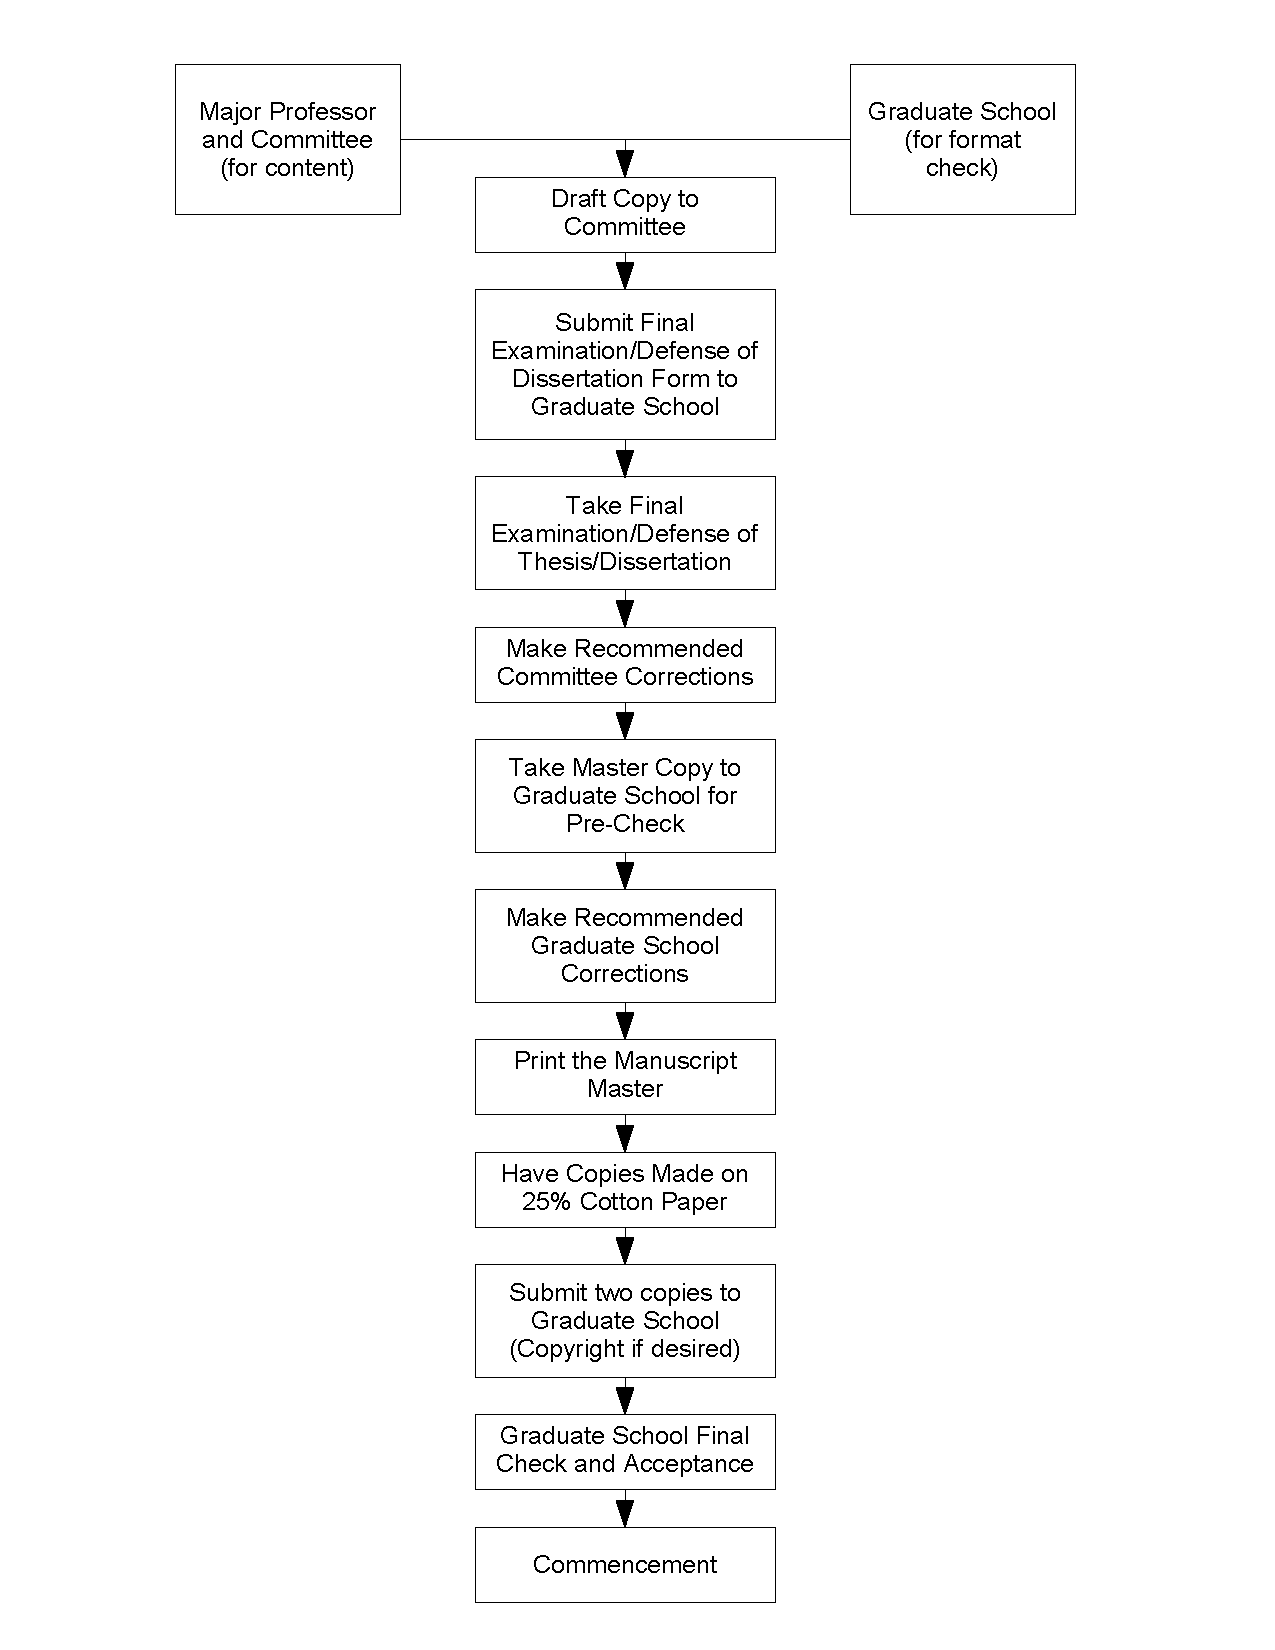
\includegraphics[width=0.9\textwidth]{thesis-manual-content/thesis-flowchart}
  \caption{Sample Flowchart Summarizing Possible Steps to Completion and Acceptance of a The\-sis/Dis\-ser\-ta\-tion}
  \label{fig:ThesisFlowchart}
\end{figure}

\section{Draft Copy to Committee}
\label{sec:DraftCopyToCommittee}

Before you submit a draft copy of your the\-sis/dis\-ser\-ta\-tion to
your committee, it should be checked out by at least your major
professor for content. His/her recommendations should be incorporated
in the draft copy that you submit to your graduate advisory committee.
\textbf{Please note that this review by your major professor is a
  crucial step, and it may need to be repeated several times.}

When your major professor is satisfied with your draft copy, you must
submit a copy to all members of your advisory committee for their
review. At the same time you should set a date, time, and place that
is convenient for all your committee members for the presentation and
final ex\-am\-i\-na\-tion/de\-fense of your
the\-sis/dis\-ser\-ta\-tion. This date should be no sooner than one
week after you submit your draft copy to them.

\subsection{Final Examination/Defense of Thesis/Dissertation}
\label{sec:FinalExaminationDefenseOfThesisDissertation}

The format of your presentation and final examination and/or defense
of your the\-sis/dis\-ser\-ta\-tion (which in some departments
requires more than one session) is set by the policy of your
department or college.  Although its length may vary with whether it
is for a thesis or dissertation, there is typically a formal oral
presentation of your research to your advisory committee and any
guests whom you or your committee members might have invited. A period
for questions normally follows. The intention of this process is to
verify your understanding of your contribution to the body of
knowledge in your research area and your general field of study.

\subsection{Committee Revisions}
\label{sec:CommitteeRevisions}

Recommendations for changes and/or additions are a natural
by\-prod\-uct of this review of your the\-sis/dis\-ser\-ta\-tion by
your entire committee and your defense of it. These should be
critically reviewed with both your major professor and the individual
committee members who made the recommendation, and incorporated as
appropriate.

\subsection{Graduate School Pre-check}
\label{sec:GraduateSchoolPrecheck}

At this point your manuscript is ready for a pre-check by the Graduate
School prior to its final approval by your advisory committee and
submission to the printer for reproduction. This pre-check will pick
up any format problems that must be corrected before the
the\-sis/dis\-ser\-ta\-tion is printed. The Graduate School must
receive, by the date published in the Bulletin, one preliminary copy
of the the\-sis/dis\-ser\-ta\-tion for pre-check. Failure to submit
the preliminary copy by the deadline will result in your removal from
the commencement list.

\section{Graduate School Revisions}
\label{sec:GraduateSchoolRevisions}

You must now make the revisions recommended by the Graduate School. If
there is any doubt about a revision, check with the Graduate School
again. This is also the appropriate time to take a copy of your
manuscript to each of your advisory committee members to obtain their
final approval of your the\-sis/dis\-ser\-ta\-tion, as reflected by
their signature on your Certificate of Approval of
The\-sis/Dis\-ser\-ta\-tion.

\section{Printing the Manuscript Master}
\label{sec:PrintingTheManuscriptMaster}

\textbf{Under no circumstances should you generate the two final
  copies from a printer.} You must photocopy them from the manuscript
master onto 25 percent cotton content, 20 pound paper. The surface of
cotton paper is such that ink from nonimpact printers does not always
adhere permanently. The general premise of most photocopying is a
combination of heat and pressure which produces a stronger permanent
bond of the ink or toner with the paper. Although some printers
function in much the same way, neither the heat or pressure is
sufficient to assure a permanent bond to 25 percent cotton paper. This
is a potential problem of all nonimpact printers. The problem has been
noted on various brands of cotton paper and with a variety of
printers. In some cases there has been flaking on random pages or
smearing of copy from pages rubbing against each other.

The printer quality should be sufficient to produce a smooth,
high-contrast copy. The poor quality of low-density dot matrix print
is not acceptable.

\section{Copying}
\label{sec:Copying}

ou will find area copy shops that are familiar with the University's
requirements concerning paper and copy quality. The cost of having
copies made by local shops is reasonable, and you will save little
money by buying your paper and doing your own copying. Professional
shops are responsible for equipment malfunctions and should maintain a
supply of 25 percent cotton paper.

All brands of 20 pound, 25 percent cotton paper are acceptable, but
all pages, including the approval sheets and any outsize pages
(11$\times$17 inches), must be on the same brand. If you are an
out-of-town student, you may wish to investigate copy shops in your
location for comparison with those in this area. Often local shops
will make arrangements to accept the master copy by mail, make the
copies, and deliver them to the Graduate School for a fee.

\section{Submission to Graduate School}
\label{sec:SubmissionToGraduateSchool}

\subsection{Official Copies}
\label{sec:OfficialCopies}

The Graduate School must receive, by the date published in the
Bulletin, two official copies of the the\-sis/dis\-ser\-ta\-tion,
including the Certificate of Approval of The\-sis/Dis\-ser\-ta\-tion
with original signatures, on 20 pound 25 percent cotton paper in an
8.5$\times$11 inch file folder. These two official copies will be
hard-bound and placed in the Tennessee Technological University
Library under arrangements made by the Graduate School. Doctoral
students must provide one additional copy for microfilming by
University Microfilms International of Ann Arbor, Michigan. This
constitutes publication and makes the dissertation available to the
public. Your department may require additional copies of your
the\-sis/dis\-ser\-ta\-tion.

\subsection{Additional Copies and Binding}
\label{sec:AdditionalCopiesAndBinding}

You are also responsible for the reproduction of all other copies of
the the\-sis/dis\-ser\-ta\-tion. Hard binding of these copies may be
arranged through the Graduate School. Your major professor can help
determine who expects to receive copies and how they should be bound.

\subsection{Copyright}
\label{sec:AssigningCopyright}

If the research work for your thesis or dissertation was supported in
part by a contract or grant, you should check with your major advisor
relative to any restrictions that might apply to copyrighting the
material. After consultation with the chairperson of your advisory
committee, you should decide whether or not to copyright the thesis to
discourage unauthorized copying. If you decide to copyright, you must
insert an extra page after the title page of each volume. Assign this
page the number ii, but do not type the number on the page. Type and
center the following information on the copyright page:
\begin{center}
  \begin{tabular}[h]{|c|} \hline
    Copyright \copyright $\underbar{\quad\quad\quad\quad\quad}$, 20 (year) \\
    All rights reserved \\ \hline
  \end{tabular}
\end{center}

Registration of your the\-sis/dis\-ser\-ta\-tion document with the
U.S.  Copyright Office is optional. Once the copyright notice is
placed in the document, it is fully protected by the Copyright Law;
however, registration is a prerequisite to certain remedies for
infringement.

In view of the University's Policy on Patents and Copyrights, with
regard to the\-sis/dis\-ser\-ta\-tion support, you should consult the
chairperson of your advisory committee before the copyright notice is
placed in the document. A copy of the University Policy is available
in the Office of Research.

\section{Graduate School Final Check and Acceptance}
\label{sec:GraduateSchoolFinalCheckAndAcceptance}

After you have submitted the final copies to the Graduate School, that
office will review your the\-sis/dis\-ser\-ta\-tion again for
corrections made on any previous errors and will count the pages. When
this review has been successfully completed, your
the\-sis/dis\-ser\-ta\-tion will be approved.

\section{Commencement}
\label{sec:Commencement}

Commencement is a fitting culmination of your effort to obtain a
graduate degree. Whatever the degree to be conferred, it marks an
appropriate beginning.

%%% Local Variables: 
%%% mode: latex
%%% TeX-master: "thesis"
%%% End: 

% Bibliography
\renewcommand{\bibname}{Bibliography} %%% If you're using BibTeX, fill out the following two commands with the name
%%% of your .bib file and the name of your .bst file. Otherwise, comment them
%%% out:

\bibliography{\jobname-content/\jobname}
\bibliographystyle{ttunatbib-mwr}
%\bibliographystyle{plain}

%%% If you're doing your bibliography manually, then uncomment the
%%% following lines and enter your bibliography entries below:

% Appendices
\renewcommand{\appendixtocname}{Appendix}
\appendix
\chapter{Sample Tables}
\label{chap:sample_tables}

\begin{table}[tbp]
  \caption{Lin Plate and Incremental Loading Method Deflections Along Free Edge in Inches}
  \label{tab:LinPlate}
  \centering
  \begin{tabular}{rrrrrr} \hline
    Total & Position & \multirow{3}{*}{Lin Plate} & \multicolumn{3}{c}{Deflections} \\
    Load & X-axis & & \multicolumn{3}{c}{Incremental Loading Method} \\
    (lbs) & (in) & & 1,49,72 & 10,49,72 & 20,169,288 \\
    \hline
    \\
    0.722 & 1.0 & -.04 & -.043 & -.046 & -.047 \\
    \\
    & 2.0 & -.16 & -.166 & -.165 & -.166 \\
    \\
    & 3.0 & -.36 & -.349 & -.331 & -.333 \\
    \\
    & 4.0 & -.56 & -.574 & -.531 & -.533 \\
    \\
    & 5.0 & -.78 & -.828 & -.753 & -.757 \\
    \\
    & 6.0 & -1.04 & -1.100 & -.992 & -1.000 \\
    \\ \hline
  \end{tabular}
\end{table}

\begin{table}[tbp]
  \caption{Means and standard errors of depths occupied by threadfin shad, alewife, and walleye in Dale Hollow Reservoir, Tennessee. Mean depths that share the same letter are not significantly different (Tukey's test; $P>0.05$)}
  \label{tab:FishDepths}
  \centering
  \begin{tabular}{llrrr} \hline
    & & & \multicolumn{2}{c}{DEPTH (m)} \\ \cline{4-5}
    SEASON & SPECIES & N & MEAN & SE \\ \hline
    Summer 1990 & Threadfin shad & 2043 & $6.6^{\textrm{a}}$ & 0.08 \\
    Summer 1990 & Alewife & 816 & $12.5^{\textrm{b}}$ & 0.13 \\
    Summer 1990 & Walleye & 22 & $10.3^{\textrm{c}}$ & 0.62 \\
    \\
    Fall 1990 & Threadfin shad & 283 & $6.7^{\textrm{a}}$ & 0.29 \\
    Fall 1990 & Alewife & 447 & $9.0^{\textrm{b}}$ & 0.33 \\
    Fall 1990 & Walleye & 26 & $10.5^{\textrm{b}}$ & 0.96 \\
    \\
    Winter 1990 & Threadfin shad & 72 & $3.0^{\textrm{a}}$ & 0.34 \\
    Winter 1990 & Alewife & 395 & $7.3^{\textrm{b}}$ & 0.31 \\
    Winter 1990 & Walleye & 13 & $10.5^{\textrm{b}}$ & 1.63 \\
    \\
    Spring 1991 & Threadfin shad & 749 & $2.7^{\textrm{a}}$ & 0.07 \\
    Spring 1991 & Alewife & 689 & $4.5^{\textrm{b}}$ & 0.08 \\
    Spring 1991 & Walleye & 3 & $4.3^{\textrm{a}}$ & 1.67 \\
    \\
    Summer 1991 & Threadfin shad & 151 & $10.5^{\textrm{a}}$ & 0.13 \\
    Summer 1991 & Alewife & 1251 & $12.3^{\textrm{b}}$ & 0.09 \\
    Summer 1991 & Walleye & 10 & $12.2^{\textrm{a}}$ & 1.16 \\
    \\
    Fall 1991 & Threadfin shad & 39 & $4.4^{\textrm{a}}$ & 0.47 \\
    Fall 1991 & Alewife & 66 & $6.3^{\textrm{b}}$ & 0.48 \\
    Fall 1991 & Walleye & 10 & $10.1^{\textrm{c}}$ & 0.77 \\
    \\ \hline
  \end{tabular}
\end{table}

\begin{sidewaystable}[tbp] 
  \caption{Meristic Characters used in Distinguishing Redeye Bass, Smallmouth Bass, and Meristic Hybrids from Roaring River, Tennessee, 1988}
  \label{tab:MeristicCharacters}
  \centering
  \begin{tabular}{lccc} \hline \hline
    \\
    & \textit{Micropterus coosae} & Meristic Hybrids & \textit{Micropterus dolomieui} \\
    & $n=32$ & $n=20$ & $n=35$ \\\
    & $x\pm$ SD & $x\pm$ SD & $x\pm$ SD \\
    Meristic & (range) & (range) & (range) \\
    \\ \hline
    \\
    Lateral line scales & $66.9 \pm 2.6$ & $71.4 \pm 1.6$ & $74.1 \pm 2.4$ \\
    & (61--71) & (70--75) & (69--79) \\
    \\
    Scales above lateral line & $8.7 \pm 0.5$ & $9.9 \pm 1.0$ & $11.8 \pm 0.7$ \\
    & (8--10) & (8--12) & (11--13) \\
    \\
    Scales below lateral line & $15.9 \pm 1.8$ & $17.5 \pm 2.4$ & $21.8 \pm 2.4$ \\
    & (11--19) & (13--21) & (14--25) \\
    \\
    Anal rays & $10.1 \pm 0.7$ & $10.7 \pm 0.7$ & $11.1 \pm 0.4$ \\
    & (9--12) & (9--12) & (10-12) \\
    \\
    Pyloric cacea & $10.8 \pm 2.0$ & $11.7 \pm 0.7$ & $11.1 \pm 0.4$ \\
    & (7--17) & (10--14) & (10--16) \\
    \\
    Meristic index & $112.2 \pm 3.7$ & $119.1 \pm 3.6$ & $131.6 \pm 4.2$ \\
    & (102--120) & (115--125) & (123--140) \\
    \\ \hline
  \end{tabular}

  \parbox{\textheight}{Source: William D. Crumby, ``Growth Dynamics of
    an Introduced Population of Redeye Bass in a North-Central
    Tennessee Stream.''  Master of Science Thesis in Biology,
    Tennessee Technological University, August 1987.}
\end{sidewaystable}

%%% Local Variables: 
%%% mode: latex
%%% TeX-master: "thesis"
%%% End: 

% Vita
\vita{\jobname-content/vita}

\end{document}
